\def\year{2020}\relax

\documentclass[letterpaper]{article}

\usepackage{aaai20}
\usepackage{times}
\usepackage{helvet}
\usepackage{courier}
\usepackage[hyphens]{url}
\usepackage{graphicx}
\urlstyle{rm}
\def\UrlFont{\rm}

\usepackage{graphicx}
\frenchspacing
\setlength{\pdfpagewidth}{8.5in}
\setlength{\pdfpageheight}{11in}

\usepackage{amsmath,amssymb,amsthm}
\usepackage[vlined,algoruled,titlenumbered,noend,portugues]{algorithm2e}
\usepackage{booktabs}

\graphicspath{{./images/}}

\pdfinfo{
  /Title (Relatório 02 - Algoritmos de Aprendizado por Reforço)
  /Author (Daniel Baptista Dias)
}

% /Title (Relatório 01 - Algoritmos de Planejamento Probabilístico)
% /Author (Daniel Baptista Dias)

\setcounter{secnumdepth}{0} %May be changed to 1 or 2 if section numbers are desired.

% The file aaai20.sty is the style file for AAAI Press proceedings, working notes, and technical reports.
\setlength\titlebox{2.5in} % If your paper contains an overfull \vbox too high warning at the beginning of the document, use this
% command to correct it. You may not alter the value below 2.5 in

\title{Relatório 02 - Algoritmos de Aprendizado por Reforço}
\author{Daniel Baptista Dias}

\begin{document}

\maketitle

\section{Introdução}
\label{sec:introducao}

Na disciplina de Inteligência Artificial existem algumas áreas que estudam formas de como um agente pode tomar um conjunto 
de decisões em sequência interagindo com um ambiente com o objetivo de solucionar um problema da melhor forma possível.

Uma forma de modelar esta situação é utilizando os Processos Markovianos de Decisão (MDP, do 
inglês \textit{Markov Decision Processes})\cite{Puterman-1994}, onde é assumido o resultado da interação do agente com o ambiente é incerto, 
e que uma ação realizada pelo agente neste ambiente em uma situação (um estado do ambiente) pode ter diferentes resultados, cuja frequência é ditada por
uma distribuição de probabilidades, e retorna uma recompensa para o agente.

No trabalho anterior o objeto de estudo foi a área de Planjemamento Probabilístico que busca dado o conhecimento de um MDP, busca encontrar qual é a 
melhor forma de agir dado cada situação possível neste ambiente. Porém em algumas situações encontrar essa melhor solução pode ser complexo, seja por 
o número de situações possíveis ser muito alto, seja por não termos muitos dados do ambiente para poder montar uma estratégia nele.

A área de Aprendizado por Reforço busca atacar esses problemas assumindo que o agente poderá interagir nesse ambiente mesmo sem um conhecimento (ilustrada pela
figura \ref{fig:rf-agent-interaction}), de forma que ele possa executar ações nele e a medida que vá interagindo com o ambiente, vá aprendendo mais características 
(estados, transições e recompensas) sobre ele e vá buscando encontrar melhores maneiras de agir.

\begin{figure}[t]
  \centering
  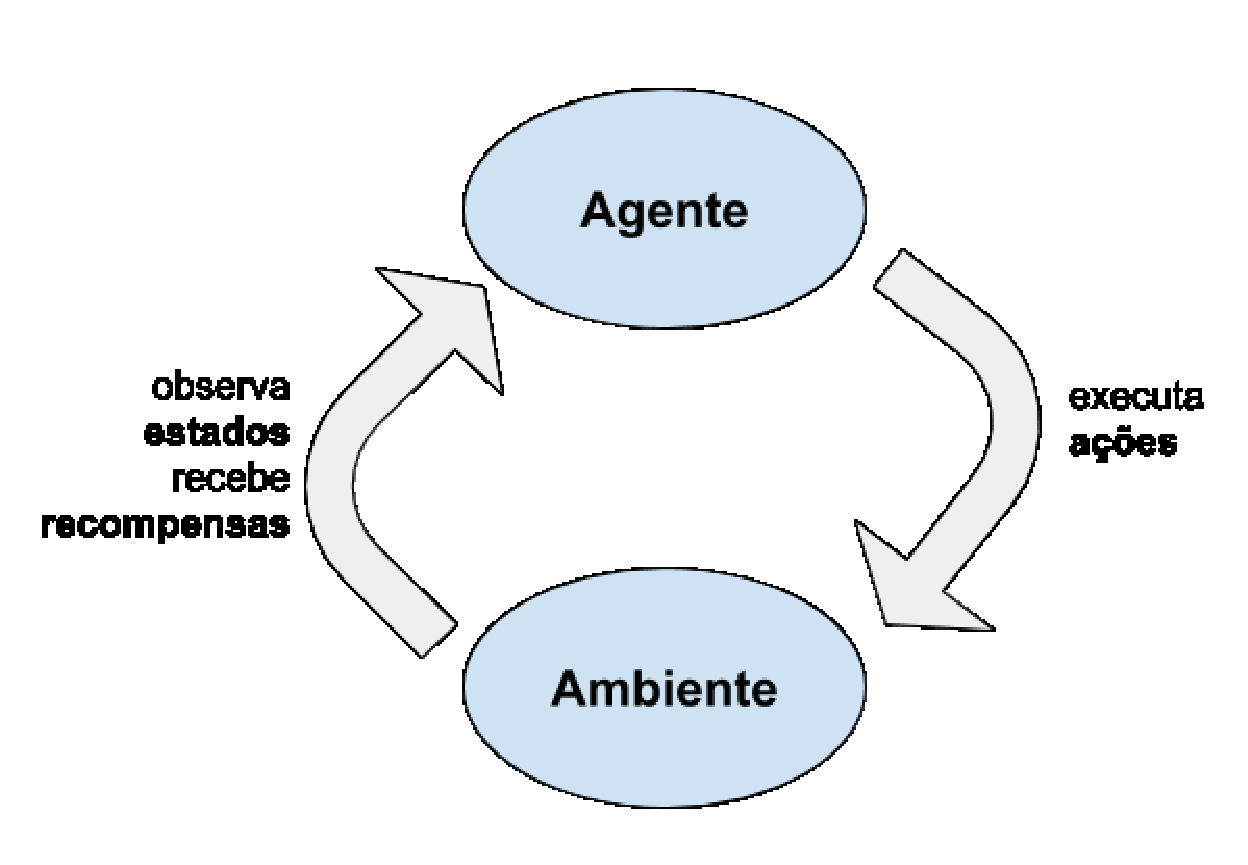
\includegraphics[width=0.9\columnwidth]{rf-agent-interaction}
  \caption{Interação de um agente com o seu ambiente}
  \label{fig:rf-agent-interaction}
\end{figure}

Neste trabalho, para efeito de estudo, serão feitos alguns experimentos com os algoritmos \textit{Q-Learning}, \textit{SARSA}, 
\textit{REINFORCE com baseline} e \textit{Fitt-Q} e seus resultados serão discutidos e comparados.

\section{Arcabouço Teórico}

No contexto de tomada de decisões por um agente em um ambiente completamente observável, um Processo de Decisão Markoviano (MDP)
pode ser descrito por uma tupla $\mathcal{M}=\langle S,A,R,P,\gamma \rangle$, onde:

\begin{itemize}
    \item $S$ é um conjunto de estados finitos e discretos, que definem a situação do ambiente em um determinado momento;
    \item $A$ é um conjunto de ações que o agente pode executar;
    \item $R : S \rightarrow \mathcal{R} $ é a função recompensa, que retorna a recompensa obtida pelo agente ao se alcançar um determinado estado;
    \item $P : S \times A \times S \rightarrow [0, 1]$ é uma função de transição que retorna a probabilidade de um agente, dado que executou uma ação $a \in A$ em um estado $s \in S$, alcançar o estado $s' \in S$. Neste trabalho uma notação que também será usada para representar essa transição é $P(s'|s,a)$.
\end{itemize}

Neste ambiente a tomada de decisão ocorre por etapas (estágios), onde o agente executa uma ação de cada vez alterando o estado 
do ambiente e recebendo uma recompensa ou sendo penalizado com um custo (recompensa negativa). Estes estágios são denominados pela 
notação $t \in \{ 1, \dots, T \} $, onde caso $T$ seja um número finito, consideramos o problema como um problema de \textbf{horizonte finito}.

O objetivo do agente neste MDP é encontrar uma política $\pi : S \rightarrow A$ que indique a melhor ação a ser tomada em cada estado $s$ a fim 
de se obter a maior recompensa possível.

Para identificar esta política pode-se calcular o valor dela para cada estado $s$ através do critério da recompensa esperada total. Esse critério 
indica o quanto de recompensa um agente pode receber em média a executar uma política $\pi$ a partir do estado $s_0 = s$ até o instante $T$ dado um 
fator de desconto $\gamma$ (limitado ao intervalo $[0, 1]$), calculada pela função valor $V : S \rightarrow \mathcal{R} $ para a política $\pi$:

\begin{equation} \label{eq:total_expected_reward}
    V_\pi(s) = E_{\pi} \left[ \sum_{t=0}^{T} \gamma^t r_t | s_0 = s \right]
\end{equation}

Uma política ótima $\pi^*$ para um MDP é aquela que tem o maior valor entre todas as outras políticas possíveis para cada estado, 
ou seja: $V_{\pi^*}(s) \geq V_{pi'}(s), \forall s,\pi'$.

O valor da política ótima $V_{\pi^*}$ pode ser encontrado a partir função valor ótima $V^* = V_{\pi^*}$ definida pela equação de Bellman \cite{Bellman-1966}, 
que encontra uma função valor que maximize as recompensas esperadas para todo $s \in S$:

\begin{equation} \label{eq:bellman_equation}
    V^*(s) = R(s) + \max_{a \in A} \left\{ \gamma \sum_{s'\in S} P(s'|s,a)V^*(s') \right\}
\end{equation}

Existem algoritmos que trabalham com essa abordagem para se obter a política ótima, usualmente resolvendo a equação de Bellman através de algoritmos de
\textit{programação dinâmica} como o \textit{Iteração de Valor} e a \textit{Iteração de Política} \cite{Howard-1960} de forma eficiente. Neles, aplicamos um operador 
de Bellman para cada estado, descrito pela equação \ref{eq:bellman_operator} abaixo: 

\begin{equation} \label{eq:bellman_operator}
  V^{t+1}(s) = (BV^t)(s) = \max_{a \in A} \left\{ Q^{t+1}(s,a) \right\}
\end{equation}

onde $ Q^{t+1}(s,a) $ é considerado uma função qualidade, definida por:

\begin{equation} \label{eq:quality_function}
  Q^{t+1}(s,a) = R(s) + \gamma \sum_{s'\in S} P(s'|s,a)V^t(s')
\end{equation}

Entretanto para alguns tipo de problema eles ter uma aplicabilidade limitada devido ao problema da \textit{maldição da dimensionalidade}: o fato que 
o número de estados pode ser proibitivamente grande dependendo da modelagem dos estados (por exemplo, caso um estado precise modelar muitas variáveis com 
diferentes combinações de valores) \cite{SuttonBarto-2018}. 

Uma forma de tentar evitar o problema do crescimento do espaço de estados é ao invés de usar um conhecimento completo do ambiente para resolver-lo,
buscar uma política ótima através do uso da experiência: a simulação ou interação de um agente agindo no ambiente em sequência, amostrando uma sequência de estados, 
ações e recompensas. Os métodos de \textit{Monte Carlo} buscam justamente fazer isso, baseando a tomada de decisão em cima das amostragens média dessa experiência ao 
invés de utilizar a equação de Bellman, obtendo uma estimativa da função valor $\hat{V}(s)$ e da função qualidade $\hat{Q}(s,a)$, concentrando o uso os recursos 
computacionais nos estados e ações mais relevantes para a resolução do problema.

Esse tipo de algoritmos garante uma solução $\epsilon$-ótima independente do tamanho do espaço de estados ($|S|$) mostrando que a probabilidade de falha de convergência
pode ser limitada segundo a desigualdade de Hoeffding \cite{Hoeffding-1994}. Nesses algoritmos é mostrando que caso haja uma quantidade suficientemente grande de episódios (amostras de um 
agente executando uma política $\pi_{\hat{Q}}$ em um ambiente) essa probabilidade de falha de convergência tende a zero. Um algoritmo que baseia nessa idéia de convergência é 
o UCT \cite{KocsisSzepesv-2006}.

Combinando as idéias dos métodos de Monte Carlo e de programação dinâmica (baseados no cálculo do operador de Bellman) o método de \textit{diferença temporal} buscam
calcular a função valor $V$ com base na experiência de um agente em um ambiente, que através da aproximação estocástica \cite{RobbinsMonro-1951}, estima a função valor
para um instante $t$, estado $s_t$, recompensa recebida $r_t$ e  uma taxa de aproximação a $V(s_t)$ (também chamada de taxa de aprendizado) $\alpha \in (0, 1])$ como:

\begin{equation} \label{eq:temporal_difference}
  V(s_t) = V(s_t) + \alpha [ r_t + \gamma V(s_{t+1}) - V(s_t) ]
\end{equation}

Dado uma política $\pi$ qualquer e um horizonte $T$, pode-se aplicar este método para avaliar esta política e encontrar $V_{\pi}$, em um algoritmo com garantia de 
convergência chamado $TD(0)$. Ele será a base para dois algoritmos que serão apresentados posteriormente, o \textit{Q-Learning} \cite{Watkins-Dayan-1992} e o 
\textit{SARSA}.

Mesmo não precisando iterar por todo o espaço de estados, armazenar e calcular $V(s)$ e $Q(s,a)$ pode demandar de muitos recursos computacionais 
(por exemplo, ao tentar armazenar um estado contínuo sem nenhuma técnica de discretização). Uma forma de resolver este problema é ao invés de trabalhar com uma 
aproximação da função valor $ \hat{V}(s, \theta) \approx V_{\pi}(s)$, onde ao invés de se armazenar os valores de $s$ serão armazenados o vetor de 
pesos $\theta \in \mathcal{R}^d$, onde $d$ seja menor que $|S|$. Nesta abordagem, os algoritmos se focarão em aprender os valores de $\theta$ de forma a encontrarem
uma política ótima para a interação com o ambiente.

\section{Algoritmos}

Neste trabalho foram implementados dois algoritmos \textit{value-based} que utilizam o método de diferença temporal para identificar 
uma política ótima em um ambiente: os algoritmos \textit{Q-Learning} \cite{Watkins-Dayan-1992} e \textit{SARSA}, um algoritmo que trabalha com busca no 
espaço de políticas, o \textit{REINFORCE com baseline} e um que trabalha com reuso de experiências (\textit{sample efficient}), o \textit{Fitt-Q} \cite{Riedmiller-2005}.

\subsection{Q-Learning}

bla

% falar sobre exploitação e exploração

\begin{equation} \label{eq:epsilon_greedy_action}
  \textsc{ChooseActionFromPolicy}(Q, \epsilon, s) = ?
\end{equation}

\begin{multline} \label{eq:time_diff_update_q_learning}
  \textsc{TimeDiff}(Q, s, a, s', \gamma, \alpha) = \\ 
      Q(s,a) + \alpha [r + \gamma max_a' Q(s', a') - Q(s,a)]
\end{multline}

%%%%%%%%%%%%%%%%%%%%%%%%%%%%%%%%%%%%%%%%%%%%%%%%%%%%%%%%%
\linesnumbered
\dontprintsemicolon
\begin{algorithm}[t!]
{
	\caption{\textsc{Q-Learning}($ env, T, \gamma, \alpha, \epsilon $)}
	\label{alg:q-learning}
    $Q(s,a) := 0, \forall s \in S, a \in A $\\

    \ParaCada{$ t \in \{ 1, \dots, T \} $}
    {
      $s := env.start()$\\

      \Enqto{$ \neg env.done() $}
      {
        $a := \textsc{ChooseActionFromPolicy}(Q, \epsilon, s) $\\
        $s', r := env.step(a)$\\
        $Q(s, a) = \textsc{TimeDiff}(Q, s, a, s', \gamma, \alpha)$\\
        $s := s'$ \\
      }
    }

    \Retorna{$Q$}
}
\end{algorithm}
%%%%%%%%%%%%%%%%%%%%%%%%%%%%%%%%%%%%%%%%%%%%%%%%%%%%%%%%%

\subsection{SARSA}

bla

\begin{multline} \label{eq:time_diff_update_sarsa}
  \textsc{TimeDiff}(Q, s, a, s', \gamma, \alpha) = \\ 
      Q(s,a) + \alpha [r + \gamma Q(s', a') - Q(s,a)]
\end{multline}

%%%%%%%%%%%%%%%%%%%%%%%%%%%%%%%%%%%%%%%%%%%%%%%%%%%%%%%%%
\linesnumbered
\dontprintsemicolon
\begin{algorithm}[t!]
{
	\caption{\textsc{SARSA}($ env, T, \gamma, \alpha, \epsilon $)}
	\label{alg:sarsa}
    $Q(s,a) := 0, \forall s \in S, a \in A $\\

    \ParaCada{$ t \in \{ 1, \dots, T \} $}
    {
      $s := env.start()$\\
      $a := \textsc{ChooseActionFromPolicy}(Q, \epsilon, s) $\\

      \Enqto{$ \neg env.done() $}
      {
        $s', r := env.step(a)$\\
        $a' := \textsc{ChooseActionFromPolicy}(Q, \epsilon, s') $\\
        $Q(s, a) = \textsc{TimeDiff}(Q, s, a, s', a', \gamma, \alpha)$\\
        $s := s'$ \\
        $a := a'$ \\
      }
    }

    \Retorna{$Q$}
}
\end{algorithm}
%%%%%%%%%%%%%%%%%%%%%%%%%%%%%%%%%%%%%%%%%%%%%%%%%%%%%%%%%

% apresentação sobre algoritmos clássicos e algoritmos por aproximação
% explicação do SARSA e do Q-Learning

\subsection{REINFORCE}

bla

% explicação sobre busca de política (gradiente)
% 343

%%%%%%%%%%%%%%%%%%%%%%%%%%%%%%%%%%%%%%%%%%%%%%%%%%%%%%%%%
\linesnumbered
\dontprintsemicolon
\begin{algorithm}[t!]
{
	\caption{\textsc{Reinforce}($ env, T, \gamma, \alpha $)}
	\label{alg:reinforce}
    inicializa $ \theta $ com valores arbitrários \\

    \ParaCada{$ episode \in \{ 1, \dots, T \} $}
    {
      $episodeSteps := \textsc{GenerateEpisode}(env, \theta)$\\

      \ParaCada{$s_t, r_t, a_t, t \in episodeSteps$}
      {
        $G := \sum_{k = t+1}^T \{ \gamma^{k-t-1} episodeSteps[k].r \}$\\
        $ \theta := \theta + \alpha \gamma^t G \nabla \ln \pi(a_t|s_t, \theta) $
      }
    }
}
\end{algorithm}
%%%%%%%%%%%%%%%%%%%%%%%%%%%%%%%%%%%%%%%%%%%%%%%%%%%%%%%%%

%%%%%%%%%%%%%%%%%%%%%%%%%%%%%%%%%%%%%%%%%%%%%%%%%%%%%%%%%
\linesnumbered
\dontprintsemicolon
\begin{algorithm}[t!]
{
	\caption{\textsc{Reinforce}($ env, T, \gamma, \alpha_{\theta}, \alpha_{w} $)}
	\label{alg:reinforce_baseline}
    inicializa $ \theta $ e $ w $ com valores arbitrários \\

    \ParaCada{$ episode \in \{ 1, \dots, T \} $}
    {
      $episodeSteps := \textsc{GenerateEpisode}(env, \theta)$\\

      \ParaCada{$s_t, r_t, a_t, t \in episodeSteps$}
      {
        $G := \sum_{k = t+1}^T \{ \gamma^{k-t-1} episodeSteps[k].r \}$\\
        $ \delta := G - \hat{v}(s_t, w) $\\
        $ w := w + \alpha_w \delta \nabla \hat{v}(s_t, w) $\\
        $ \theta := \theta + \alpha_{\theta} \gamma^t \delta \nabla \ln \pi(a_t|s_t, \theta) $
      }
    }
}
\end{algorithm}
%%%%%%%%%%%%%%%%%%%%%%%%%%%%%%%%%%%%%%%%%%%%%%%%%%%%%%%%%

% apresentação sobre algoritmos por policy search
% explicação do REINFORCE

\subsection{FittQ}

% sample efficient, explicar da lógica do dyna

bla
% apresentação sobre algoritmos por sample efficient
% explicação do FittQ

\begin{equation} \label{eq:msbe}
  \textsc{MSBE}(\theta, \theta') = || \hat{V}_{\theta} - \mathcal{T} \hat{V}_{\theta'} ||^2_D
\end{equation}

%%%%%%%%%%%%%%%%%%%%%%%%%%%%%%%%%%%%%%%%%%%%%%%%%%%%%%%%%
\linesnumbered
\dontprintsemicolon
\begin{algorithm}[t!]
{
	\caption{\textsc{FittQ}($ env, T, \epsilon $)}
	\label{alg:reinforce}
    inicializa $ w_0 $ com valores arbitrários \\

    \ParaCada{$ episode \in \{ 1, \dots, T \} $}
    {
      $w_t := \arg \min_{w \in \mathcal{R}^k} \textsc{MSBE}(w, w_{t-1}) $ \\
      $res := || w_t - w_{t-1} ||$ \\

      \Se{$res < \epsilon$}
      {
        \textbf{interrompe loop}
      }
    }
}
\end{algorithm}
%%%%%%%%%%%%%%%%%%%%%%%%%%%%%%%%%%%%%%%%%%%%%%%%%%%%%%%%%

\section{Experimentos e Resultados}

Uma vez implementado os algoritmos, foram elaborados alguns experimentos visando analizar a execução dos algoritmos e o comportamento deles.

Os experimentos foram executados na plataforma Google Colab com o Python, na época deste relatório com 2 CPUs de 2.2 GHz e 13GB de memória.
Parte dos algoritmos foi baseado em implementações existentes e estão disponíveis no Github\footnote{Disponível em https://github.com/danielbdias/automated-planning-and-reinforcement-learning-studies}.
Os algoritmos base das implementações foram:

\begin{itemize}
  \item \textit{Q-Learning} e \textit{SARSA}: https://github.com/dennybritz/reinforcement-learning/tree/master/TD
  \item \textit{REINFORCE}: https://github.com/SwamyDev/reinforcement
  \item \textit{FittQ}: https://github.com/seungjaeryanlee/implementations-nfq
\end{itemize}

falar sobre o PoleCart problem

bla
% TODO: avaliar experimentos e resultados

\section{Conclusão}

bla
% TODO: avaliar experimentos e resultados

\bibliography{references.bib}
\bibliographystyle{aaai}

\end{document}
